\documentclass[12pt, titlepage]{article}

% basics
\usepackage[utf8]{inputenc}

\usepackage{textcomp}
% \usepackage[dutch]{babel}
\usepackage{url}
% \usepackage{hyperref}
% \hypersetup{
%     colorlinks,
%     linkcolor={black},
%     citecolor={black},
%     urlcolor={blue!80!black}
% }
\usepackage{graphicx}
\usepackage{float}
\usepackage{booktabs}
\usepackage{enumitem}
% \usepackage{parskip}
\usepackage{emptypage}
\usepackage{subcaption}
\usepackage{multicol}
\usepackage[usenames,dvipsnames]{xcolor}

% \usepackage{cmbright}

\usepackage{amsmath, amsfonts, mathtools, amsthm, amssymb}
\usepackage{mathrsfs}
\usepackage{cancel}
\usepackage{bm}
\newcommand\N{\ensuremath{\mathbb{N}}}
\newcommand\R{\ensuremath{\mathbb{R}}}
\newcommand\Z{\ensuremath{\mathbb{Z}}}
\renewcommand\O{\ensuremath{\emptyset}}
\newcommand\Q{\ensuremath{\mathbb{Q}}}
\newcommand\C{\ensuremath{\mathbb{C}}}
\DeclareMathOperator{\sgn}{sgn}
\usepackage{systeme}
\let\svlim\lim\def\lim{\svlim\limits}
\let\implies\Rightarrow
\let\impliedby\Leftarrow
\let\iff\Leftrightarrow
\let\epsilon\varepsilon
\usepackage{stmaryrd} % for \lightning
\newcommand\contra{\scalebox{1.1}{$\lightning$}}
% \let\phi\varphi
% theorems
\makeatother
\usepackage{thmtools}
\usepackage[framemethod=TikZ]{mdframed}
\mdfsetup{skipabove=1em,skipbelow=0em}

\definecolor{geyecolor}{RGB}{199,237,204}%
\theoremstyle{definition}

\declaretheoremstyle[
    headfont=\bfseries\sffamily\color{ForestGreen!70!black}, 
    numbered=no,
    mdframed={
        linewidth=3pt,
        rightline=false, topline=false, bottomline=false,
        linecolor=ForestGreen, backgroundcolor=ForestGreen!1,
    }
]{thmgreenbox}

\declaretheoremstyle[
    headfont=\bfseries\sffamily\color{NavyBlue!70!black}, 
    numbered=no,
    mdframed={
        linewidth=2pt,
        rightline=false, topline=false, bottomline=false,
        linecolor=NavyBlue, backgroundcolor=NavyBlue!1,
    }
]{thmbluebox}

% Algoritmo.
\declaretheoremstyle[
    headfont=\bfseries\sffamily\color{OliveGreen!70!black}, 
    numbered=no,
    mdframed={
        linewidth=2pt,
        rightline=false, topline=false, bottomline=false,
        linecolor=OliveGreen, backgroundcolor=OliveGreen!1,
    }
]{thmorangealgo}

\declaretheoremstyle[
    headfont=\bfseries\sffamily\color{NavyBlue!70!black},
    numbered=no, 
    mdframed={
        linewidth=2pt,
        rightline=false, topline=false, bottomline=false,
        linecolor=NavyBlue
    }
]{thmblueline}

\declaretheoremstyle[
    headfont=\bfseries\sffamily\color{RawSienna!70!black}, 
    mdframed={
        linewidth=2pt,
        rightline=false, topline=false, bottomline=false,
        linecolor=RawSienna, backgroundcolor=RawSienna!1,
    }
]{thmredbox}

\declaretheoremstyle[
    headfont=\bfseries\sffamily\color{RawSienna!70!black}, 
    numbered=no,
    mdframed={
        linewidth=2pt,
        rightline=false, topline=false, bottomline=false,
        linecolor=RawSienna, backgroundcolor=RawSienna!1,
    },
]{thmproofbox}

\declaretheoremstyle[
    headfont=\bfseries\sffamily\color{NavyBlue!70!black}, 
    numbered=no,
    mdframed={
        linewidth=2pt,
        rightline=false, topline=false, bottomline=false,
        linecolor=NavyBlue, backgroundcolor=NavyBlue!1,
    },
]{thmexplanationbox}


\declaretheorem[style=thmgreenbox, name=Definizione]{definition}
\declaretheorem[style=thmbluebox, numbered=no, name=Esempio]{es}
\declaretheorem[style=thmbluebox, numbered=no, name=Conseguenza]{conseguenza}
\declaretheorem[style=thmredbox, name=Proposizione]{prop}
\declaretheorem[style=thmredbox, numbered=no, name=Interpretazione]{interpretazione}
\declaretheorem[style=thmredbox, name=Teorema]{theorem}
\declaretheorem[style=thmredbox, name=Esercizio]{esercizio}
\declaretheorem[style=thmorangealgo, name=Soluzione]{sol}
\declaretheorem[style=thmredbox, numbered=no, name=Lemma]{lemma}
\declaretheorem[style=thmredbox, numbered=no, name=Corollario]{corollary}
\declaretheorem[style=thmorangealgo, numbered=no, name=Algoritmo]{algo}

\declaretheorem[style=thmproofbox, name=Dimostrazione]{replacementproof}
\renewenvironment{proof}[1][\proofname]{\vspace{-10pt}\begin{replacementproof}}{\end{replacementproof}}


\declaretheorem[style=thmexplanationbox, name=Dimostrazione]{tmpexplanation}
\newenvironment{explanation}[1][]{\vspace{-10pt}\begin{tmpexplanation}}{\end{tmpexplanation}}

\declaretheorem[style=thmblueline, numbered=no, name=Ricorda]{remark}
\declaretheorem[style=thmblueline, numbered=no, name=Nota]{note}
\declaretheorem[style=thmblueline, numbered=no, name=Osservazione]{obs}

\newtheorem*{uovt}{UOVT}
\newtheorem*{notation}{Notation}
\newtheorem*{previouslyseen}{As previously seen}
\newtheorem*{problem}{Problem}
\newtheorem*{observe}{Observe}
\newtheorem*{property}{Property}
\newtheorem*{intuition}{Intuition}


\usepackage{etoolbox}
\AtEndEnvironment{vb}{\null\hfill$\diamond$}%
\AtEndEnvironment{intermezzo}{\null\hfill$\diamond$}%
% \AtEndEnvironment{opmerking}{\null\hfill$\diamond$}%

% http://tex.stackexchange.com/questions/22119/how-can-i-change-the-spacing-before-theorems-with-amsthm
\makeatletter
% \def\thm@space@setup{%
%   \thm@preskip=\parskip \thm@postskip=0pt
% }

\newcommand{\oefening}[1]{%
    \def\@oefening{#1}%
    \subsection*{Oefening #1}
}

\newcommand{\suboefening}[1]{%
    \subsubsection*{Oefening \@oefening.#1}
}

\newcommand{\exercise}[1]{%
    \def\@exercise{#1}%
    \subsection*{Exercise #1}
}

\newcommand{\subexercise}[1]{%
    \subsubsection*{Exercise \@exercise.#1}
}


\usepackage{xifthen}

\def\testdateparts#1{\dateparts#1\relax}
\def\dateparts#1 #2 #3 #4 #5\relax{
    \marginpar{\small\textsf{\mbox{#1 #2 #3 #5}}}
}

\def\@lesson{}%
\newcommand{\lesson}[3]{
    \ifthenelse{\isempty{#3}}{%
        \def\@lesson{Lecture #1}%
    }{%
        \def\@lesson{Lecture #1: #3}%
    }%
    \subsection*{\@lesson}
    \testdateparts{#2}
}

% \renewcommand\date[1]{\marginpar{#1}}


\usepackage[a4paper,width=165mm,top=20mm,bottom=20mm,bindingoffset=6mm]{geometry}
\usepackage[utf8]{inputenc}
\usepackage[italian]{babel}
\usepackage[OT1]{fontenc}
\usepackage{graphicx}
\usepackage{float}
\usepackage{fancyhdr}
\usepackage{xcolor}
\usepackage{mathtools}
\usepackage{amsmath}
\usepackage{amssymb}
\usepackage{tikz}
\usepackage{imakeidx}
\usepackage{textcomp}
\usepackage{pifont}
\usepackage{polynom}
\usepackage{algorithm}
\usepackage{algpseudocode}
\usepackage{mathtools}
\usepackage[colorlinks=true,linkcolor=black,anchorcolor=black,citecolor=black,filecolor=black,menucolor=black,runcolor=black,urlcolor=black]{hyperref}
\usepackage{cancel}
\usepackage{pgfplots}
\usepackage{tabularx}

\colorlet{punct}{red!60!black}
\definecolor{background}{HTML}{EEEEEE}
\definecolor{delim}{RGB}{20,105,176}
\colorlet{numb}{magenta!60!black}
\pagestyle{fancy}
\everymath{\displaystyle}


\begin{document}
  \begin{titlepage}
    \begin{center}
        
\includegraphics[width=0.4\textwidth]{img/logo_uniba}\\
        \vspace{1cm}
        % Dipartimento
        {\large Dipartimento di Informatica}\\
        \vspace{1cm}
        % Corso di laurea
        {\large Corso di laurea in Informatica}\\
        \hrulefill \\
        \vspace{2cm}
        {\large \textbf{Metodi Avanzati di Programmazione}}\\
        \vspace{0.5cm}
        % Materia
        {\large Kmeans}\\
        \vspace{2cm}
        % Titolo
        {\LARGE\textbf{Documentazione}}\\
        \vspace{2cm}

        \vfill
        
    
        \begin{table}[ht]
          \centering
          \begin{tabularx}{\textwidth}{@{}X@{}}
              Progetto di: \\
              \textbf{Davide Cirilli} (760412) \href{mailto:d.cirilli2@studenti.uniba.it}{d.cirilli2@studenti.uniba.it} \\
              \textbf{Mattia Curri} (758306) \href{mailto:m.curri8@studenti.uniba.it}{m.curri8@studenti.uniba.it} \\
              \textbf{Emanuele Fontana} (758344) \href{mailto:emanuele.fontana7@studenti.uniba.it}{emanuele.fontana7@studenti.uniba.it}\\
          \end{tabularx}
      \end{table}

        \vspace{1cm}
        \hrulefill \\
        \vspace{1cm}
        % Anno accademico in cui si è iscritti
        {\large Anno Accademico \textbf{2022-2023}}
    \end{center}
\end{titlepage}
  \tableofcontents
  \newpage
  \section{Introduzione}

Il programma sviluppato fa uso dell'algoritmo di clustering \textbf{\textit{K-means}} per analizzare informazioni estratte da tabelle di un database, sfruttando il servizio MySQL.

Il \textit{K-means} è un algoritmo di clustering, una tecnica di apprendimento non supervisionato utilizzata per suddividere un insieme di dati in gruppi omogenei chiamati \textit{cluster}. 
L'obiettivo del \textit{K-means} è di assegnare ogni dato al cluster più vicino, in modo che i punti all'interno di ciascun cluster siano simili tra loro e i punti tra cluster diversi siano diversi. 
Ecco come funziona l'algoritmo \textit{K-means}: 
\begin{enumerate}
  \item \textbf{Inizializzazione}: Si inizia scegliendo il numero \textit{k} desiderato di \textit{cluster}. L'algoritmo crea \textit{k} partizioni e assegna casualmente \textit{k} punti come centroidi iniziali, uno per partizione. Un centroide rappresenta il centro del \textit{cluster}.
  \item \textbf{Assegnazione}: Ciascuna transazione viene assegnata al suo \textit{cluster}. L'appartenenza  dipende dalla distanza della transazione dal centroide del \textit{cluster}, l'obiettivo è minimizzare la distanza tra centroide e transazione.
  \item \textbf{Aggiornamento dei centroidi}: Una volta assegnati tutti i punti ai \textit{cluster}, i centroidi vengono aggiornati calcolando la media delle posizioni dei punti all'interno di ciascun \textit{cluster}. Questa media diventa il nuovo centroide per il \textit{cluster} corrispondente.
  \item \textbf{Ripetizione}: I passi 2 e 3 vengono ripetuti fino a quando i centroidi smettono di cambiare o si raggiunge un numero massimo di iterazioni.
  \item \textbf{Risultato}: Alla fine delle iterazioni si ottiene un insieme di \textit{k} \textit{cluster} e ogni transazione sarà stata assegnata al \textit{cluster} più vicino.
\end{enumerate}

\noindent È importante notare che il risultato finale può variare a seconda della scelta iniziale dei centroidi. In alcuni casi, l'algoritmo può convergere verso un minimo locale anziché verso il risultato ottimale. 
  \newpage
  
  \section{Features}
\subsection{Progetto Base}
\noindent La versione base del progetto consiste in un'architettura client/server che permette all'utente la scoperta/lettura di cluster. Il server dovrà essere eseguito su una macchina con un database MySQL in esecuzione. 
Il servizio sara' raggiungibile sulla porta 8080, e potrà comunicare con diversi client contemporaneamente. 
\\ I servizi offerti dal server all'utente tramite il client CLI sono i seguenti:
\begin{itemize}[label=-]
  \item \textbf{lettura di cluster} fornendo al server il path del file in cui sono savati i cluster da recuperare 
  \item \textbf{scoperta di cluster} fornendo al server il nome della tabella presente nel database ed il numero di cluster da scoprire
  \item \textbf{salvataggio dei cluster} generati nella macchina dove il server viene eseguito, dove potranno essere successivamente letti. 
\end{itemize}
Il server salverà informazioni relativi agli errori nel file di logging mentre nell'interfaccia CLI notificherà l'utente quando la comunicazione si interrompe o se vi sono problemi con gli input dati. Il client da riga di comando permette di collegarsi ad una macchina che sta eseguendo un'istanza del server. L'utente nel menù avra le due opzioni di lettura o scoperta di cluster, mentre il salvataggio avverrà in automatico lato server alla generazione di nuovi cluster.

\subsection{Estensione}
  \newpage
  
  \section{Installazione e avvio}
\subsection{Requisiti Server}
\subsubsection{Base}
\noindent Per utilizzare il server è necessario:
\begin{itemize}[label=-]
  \item Installare \href{https://dev.mysql.com/downloads/installer/}{MySQL} sul proprio computer
  \item Eseguire lo script sql presente nel percorso "\textbackslash KmeansServer\textbackslash out\textbackslash artifacts\textbackslash KmeansServer\_jar"
  \item Installare \href{https://www.oracle.com/technetwork/java/javase/downloads/jre8-downloads-2133155.html}{JRE} 8
  \item Installare JDK 19.0.2
\end{itemize}

\subsubsection{Estensione}


\subsection{Requisiti Client}
\subsubsection{CLI}
\noindent Per utilizzare il client è necessario:
\begin{itemize}[label=-]
  \item Installare \href{https://www.oracle.com/technetwork/java/javase/downloads/jre8-downloads-2133155.html}{JRE} 8  
  \item Server in ascolto
\end{itemize}

\subsubsection{App}
\noindent Per utilizzare il client app è necessario:
\begin{itemize}[label=-]
  \item Un dispositivo Android con sistema operativo Android 5.0 Lollipop o superiore
  \item Installare l'applicazione: trasferire l'APK sullo smartphone (\textbf{percorso APK}). Aprire il file APK e installare l'applicazione. Se necessario abilitare l'installazione di applicazioni da sorgenti sconosciute e dare l'ok nel caso in cui l'installazione venga bloccata da Play Protect.
  \item Server in ascolto
\end{itemize}


\subsection{Avvio server}
\subsubsection{CLI}
\noindent Per avviare il server e' necessario eseguire il file \textit{server.bat} nella stessa cartella di \textit{server.jar}. In alternativa è possibile avviarlo da riga di comando tramite il comando \textit{java -jar server.jar}.

\subsubsection{App}
\noindent

\subsection{Avvio client}
\subsubsection{CLI}
\noindent Per avviare il client da riga di comando è necessario eseguire il file \textit{client.bat} nella stessa cartella del file \textit{client.jar}. Questa modalità di avvio connetterà il client ad un server in esecuzione sulla propria macchina sulla porta 8080. Per specificare un altro server a cui connettersi è necessario
avviare il client da riga di comando tramite il comando \textit{java -jar client.jar indirizzo\_ip porta} o inserendo tale comando nel file batch.


\subsubsection{App}
\noindent Per avviare il client app basta avviare l'applicazione sul proprio smartphone ed inserire indirizzo ip e porta del server a cui ci si vuole connettere:
\begin{figure}[H]
  \centering
  
\includegraphics[scale=0.25]{img/app1.png}
  \caption{Schermata iniziale dell'applicazione}
\end{figure}

  \newpage
  
  \section{Esempi di test (CLI)}
\begin{enumerate}
  \item \textbf{Esecuzione del client con server offline} \\ \\
  \begin{minipage}[t]{0.3\textwidth}
    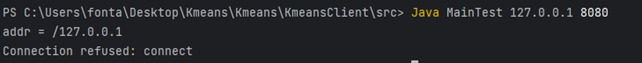
\includegraphics[scale=0.8]{img/test1.png}
  \end{minipage}
  \item \textbf{Esecuzione senza parametri}: il programma deve essere avviato fornendo come parametri l'indirizzo IP/DNS del server e la porta logica. Se si lavora con la stessa macchina si può inserire come primo parametro localhost, 127.0.0.1 (indirizzo IPv4 locale) oppure ::1 (indirizzo IPv6 locale). \\ \\
  \begin{minipage}[t]{0.3\textwidth}
    
\includegraphics[scale=0.8]{img/test2.png}
  \end{minipage}
  \item \textbf{Esecuzione con porta errata}: la porta logica è un numero a 16 bit, dunque un decimale compreso tra 0 e 65.535. \\ \\
  \begin{minipage}[t]{0.3\textwidth}
    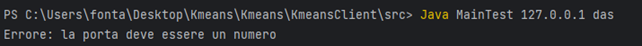
\includegraphics[scale=0.8]{img/test3.png}
  \end{minipage}
  \item \textbf{Esecuzione con IP/DNS inesistente}: in questa esecuzione il server non esiste e dunque il client non riesce a connettersi. In particolare il programma si connette a un server DNS per convertire l'indirizzo fornito in un indirizzo IP ma tale indirizzo non è registrato e dunque si ha errore. \\ \\
  \begin{minipage}[t]{0.3\textwidth}
    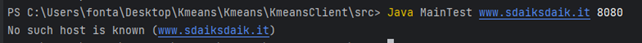
\includegraphics[scale=0.8]{img/test4.png}
  \end{minipage}
  \item \textbf{Esecuzione con parametri corretti}: quando il programma viene eseguito nelle condizioni funzionali (quindi server avviato e parametri validi) vengono stampati a schermo indirizzo IP e porta del server, seguiti dalla porta che sta usando il processo per la comunicazione. Viene poi mostrato all'utente un menù con due opzioni. L'opzione (1) permetterà al client di caricare un cluster di dati che è stato serializzato sul server come un file, mentre l'opzione (2) consente di creare un nuovo cluster di dati mediante l'algoritmo del K-means. In caso di input non validi viene chiesto all'utente di reinserire finchè non si avrà un'opzione valida.  \\ \\
  \begin{minipage}[t]{0.3\textwidth}
    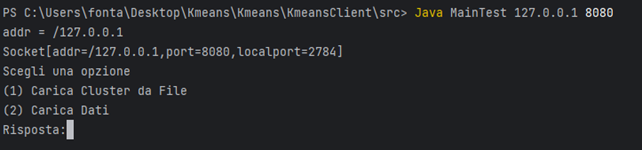
\includegraphics[scale=0.8]{img/test5.png}
  \end{minipage}
  \\
  \begin{minipage}[t]{0.3\textwidth}
    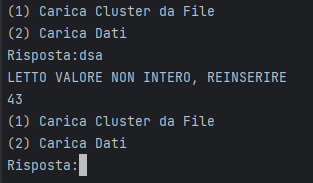
\includegraphics[scale=0.8]{img/test6.png}
  \end{minipage}
  \begin{itemize}[label=-]
    \item \textbf{Opzione (1)}: Viene chiesto all'utente di inserire il nome del database, della tabella e del numero di cluster creati. Il server andrà dunque a cercare il file corrispondente a tali informazioni e, se non trovato, manderà un messaggio di errore all'utente (come nell'esempio). Viene chiesto all'utente se vuole tornare al menù oppure terminare l'esecuzione del programma. Se viene digitato \textit{n} il programma termina. Nel caso in cui il file corrispondente alle richieste esista viene inviato al client il contenuto del file, ovvero i centroidi dei cluster. \\ \\
    \begin{minipage}[t]{0.3\textwidth}
      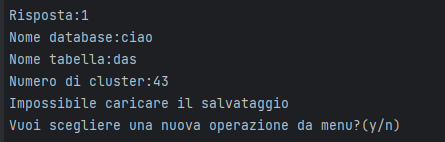
\includegraphics[scale=0.8]{img/test7.png}
    \end{minipage}
    \\
    \begin{minipage}[t]{0.3\textwidth}
      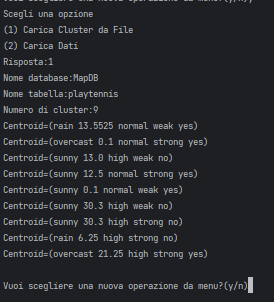
\includegraphics[scale=0.8]{img/test8.png}
    \end{minipage}
    \item \textbf{Opzione (2)}: Viene chiesto all'utente se vuole usare i valori di default o meno:
    \begin{itemize}[label=-]
      \item \textbf{Valori di default}: i valori di default sono:
      \begin{itemize}[label=-]
        \item localhost $\rightarrow$ server database
        \item 3306 $\rightarrow$ porta dabasase
        \item MapDB $\rightarrow$ nome database
        \item playtennis $\rightarrow$ nome tabella
        \item MapUser $\rightarrow$ nome utente
        \item password di MapUser
      \end{itemize}
      \begin{minipage}[t]{0.3\textwidth}
        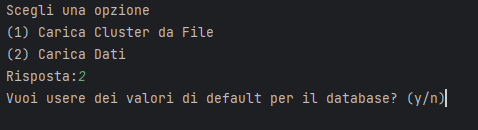
\includegraphics[scale=0.8]{img/test9.png}
      \end{minipage}
      \\ Nel caso di risposta affermativa viene chiesto all'utente il numero dei cluster. Una volta confermati (se questi sono validi) il server eseguirà l'algoritmo di K-means e invierà il risultato al client. Viene poi chiesto se si vuole riprendere l'esecuzione sullo stesso dataset o meno. \\ \\
      \begin{minipage}[t]{0.3\textwidth}
        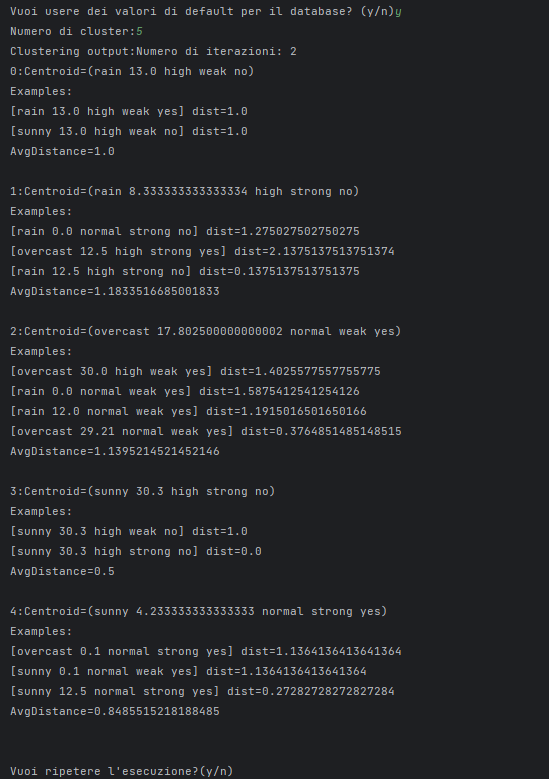
\includegraphics[scale=0.8]{img/test10.png}
      \end{minipage}
      \\ Se l'utente non vuole ripetere l'esecuzione sul dataset ha due scelte:
      \begin{enumerate}
        \item Tornare al menù
        \item Terminare l'esecuzione
      \end{enumerate}
      \begin{minipage}[t]{0.3\textwidth}
        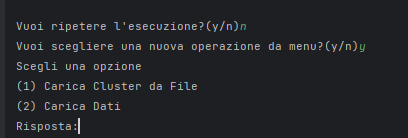
\includegraphics[scale=0.8]{img/test12.png}
      \end{minipage}
      \item \textbf{Valori non di default}: l'utente può scegliere di non usare i valori di default. In quel caso deve inserire tutte le informazioni necessarie. In caso di valori non validi verrà segnalato l'errore all'utente, il quale sceglierà se proseguire con i valori di default oppure se riprovare a inserire dei valori personalizzati. L'uso di valori personalizzati permette di utilizzare dataset già presenti nel server del database. \\ \\
      \begin{minipage}[t]{0.3\textwidth}
        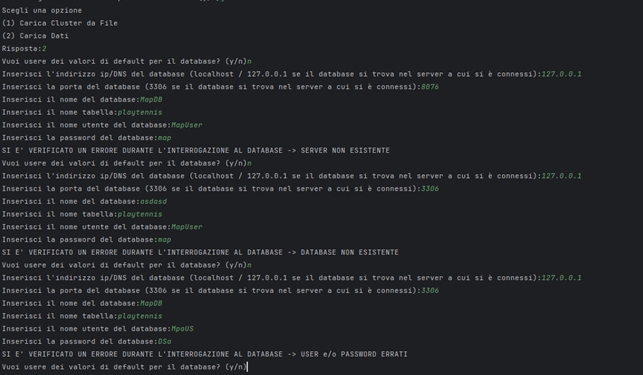
\includegraphics[scale=0.8]{img/test13.png}
      \end{minipage}
    \end{itemize} 
    Ogni volta che l'utente richiede la creazione di un dataset al server, quest'ultimo serializzerà i cluster in un file con nome del tipo: \textbf{\textit{NomedatabaseNometabellaNumerocluster.dat}}. \\ \\
    \begin{minipage}[t]{0.3\textwidth}
      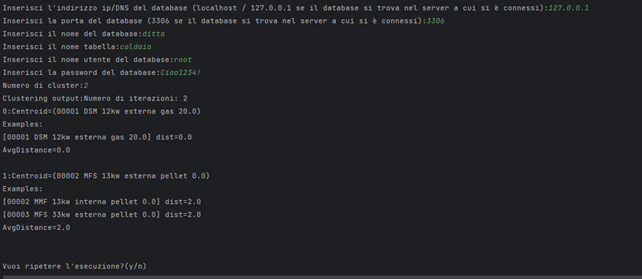
\includegraphics[scale=0.8]{img/test14.png}
    \end{minipage}
  \end{itemize}
\end{enumerate}
\end{document}